\documentclass[english]{article}

\usepackage[latin9]{inputenc}
\usepackage[letterpaper]{geometry}
\geometry{verbose,tmargin=1in,bmargin=1in,lmargin=1in,rmargin=1in}
\usepackage{amsmath}
\usepackage{tikz}
\usetikzlibrary{automata,positioning}

\tikzstyle{dir}=[->, very thick]
\tikzstyle{circ}=[draw, circle, very thick]

\title{CIS 511 Homework 1}
\author{Stephen Phillips, Daegan Golomb}
\date{\today }


\begin{document}
\maketitle
\subsection*{Problem 1}

\subsubsection*{(c)}
Here the states $q_{ij}$ mean we have see $i$ (mod 2) $a$ symbols and $j$ b symbols (until 3 where we stop counting).

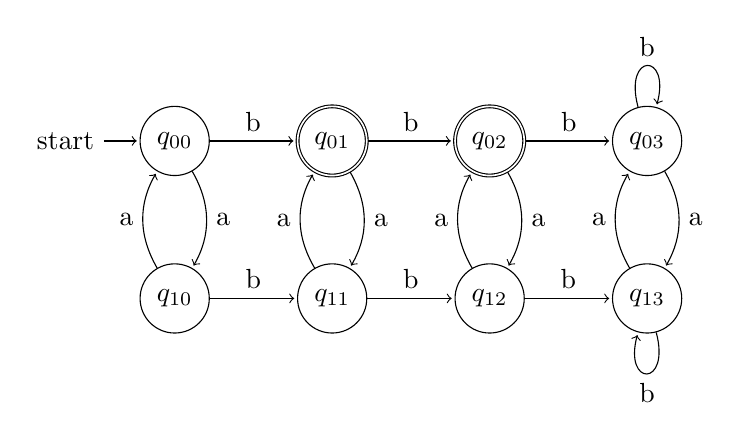
\begin{tikzpicture}[shorten >=1pt,node distance=2cm,on grid,auto] 
   \node[state,initial] (q_00)   {$q_{00}$}; 
   \node[state,accepting] (q_01) [right=of q_00] {$q_{01}$}; 
   \node[state,accepting] (q_02) [right=of q_01] {$q_{02}$};
   \node[state] (q_03) [right=of q_02] {$q_{03}$}; 
   \node[state](q_10) [below=of q_00] {$q_{10}$};
   \node[state](q_11) [right=of q_10] {$q_{11}$};
   \node[state](q_12) [right=of q_11] {$q_{12}$};
   \node[state](q_13) [right=of q_12] {$q_{13}$};
    \path[->] 
    (q_00) edge  node {b} (q_01)
          edge[bend left]  node  {a} (q_10)
    (q_01) edge  node {b} (q_02)
          edge[bend left]  node  {a} (q_11)
    (q_02) edge  node {b} (q_03)
          edge[bend left]  node  {a} (q_12)
    (q_03) edge [loop above] node {b} ()
          edge[bend left]  node {a} (q_13) 
    (q_10) edge  node {b} (q_11)
          edge[bend left]  node  {a} (q_00)
    (q_11) edge  node {b} (q_12)
          edge[bend left]  node  {a} (q_01)
    (q_12) edge  node {b} (q_13)
          edge[bend left]  node  {a} (q_02)
    (q_13) edge [loop below] node {b} ()
          edge[bend left]  node {a} (q_03);
\end{tikzpicture}

\subsubsection*{(g)}
Here the states $q_{ij}$ mean we have see $i$ (mod 2) total symbols and $j$ (mod 2) $a$ symbols. The top row is reversed to make the transitions more clear.

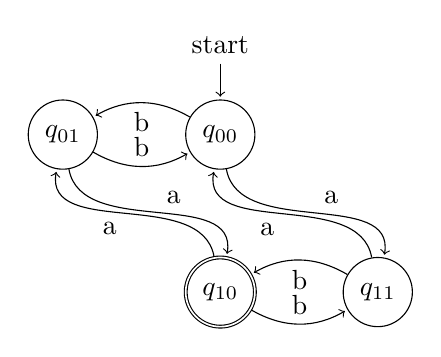
\begin{tikzpicture}[shorten >=1pt,node distance=2cm,on grid,auto] 
   \node[state,initial,initial where=above] (q_00)   {$q_{00}$}; 
   \node[state] (q_01) [left=of q_00] {$q_{01}$}; 
   \node[state,accepting](q_10) [below=of q_00] {$q_{10}$};
   \node[state](q_11) [right=of q_10] {$q_{11}$};
    \path[->] 
    (q_00) edge[bend right]  node {b} (q_01)
          edge[out=280,in=80]  node  {a} (q_11)
    (q_01) edge[bend right]  node {b} (q_00)
          edge[out=280,in=80]  node  {a} (q_10)
    (q_10) edge[bend right]  node {b} (q_11)
          edge[out=100,in=260]  node  {a} (q_01)
    (q_11) edge[bend right]  node {b} (q_10)
          edge[out=100,in=260]  node  {a} (q_00);
\end{tikzpicture}
%\begin{tikzpicture}[shorten >=1pt,node distance=2cm,on grid,auto] 
%   \node[state,initial] (q_0)   {$q_0$}; 
%   \node[state] (q_1) [above right=of q_0] {$q_1$}; 
%   \node[state] (q_2) [below right=of q_0] {$q_2$}; 
%   \node[state,accepting](q_3) [below right=of q_1] {$q_3$};
%    \path[->] 
%    (q_0) edge  node {0} (q_1)
%          edge  node [swap] {1} (q_2)
%    (q_1) edge  node  {1} (q_3)
%          edge [loop above] node {0} ()
%    (q_2) edge  node [swap] {0} (q_3) 
%          edge [loop below] node {1} ();
%\end{tikzpicture}

\subsection*{Problem 2}
\subsubsection*{(a)}
Using the method we did in class, we need to find $R_{ij}^k$ for $i,j \in \{0,1,2\}, k \in \{1,2\}$

\begin{align*}
R_{11}^{0} &=\; a \\
R_{12}^{0} &=\; b \\
R_{21}^{0} &=\; b \\
R_{22}^{0} &=\; a \\
R_{11}^{1} &=\; R_{11}^0 \cup R_{11}^0 R_{11}^{0*} R_{11}^0 = a \cup (a a^{*} a) \\
R_{12}^{1} &=\; R_{12}^0 \cup R_{11}^0 R_{11}^{0*} R_{12}^0 = b \cup (a a^{*} b) \\
R_{21}^{1} &=\; R_{21}^0 \cup R_{21}^0 R_{11}^{0*} R_{11}^0 = b \cup (b a^{*} a) \\
R_{22}^{1} &=\; R_{22}^0 \cup R_{21}^0 R_{11}^{0*} R_{12}^0 = a \cup (b a^{*} b) \\
R_{12}^{2} &=\; R_{12}^1 \cup R_{12}^1 R_{22}^{1*} R_{22}^1 = (b \cup a a^{*} b) \cup (b (a \cup b a^{*} b)^{*} (a \cup (b a^{*} b))) \\
\end{align*}


\end{document}
